%%%%%%%%%%%%%%%%%%%%%%%%%%%%%%%%%%%
% Key                | Occurences | 
%--------------------+------------| 
% Cancellieri_2010   |         10 | 
% Wouters_2010 (*)   |          5 | 
% Astrakharchik_2004 |          5 | 
% Ciuti_2005         |          5 | 
% Amo_2009 (*)       |          4 | 
%%%%%%%%%%%%%%%%%%%%%%%%%%%%%%%%%%%


\chapter{Drag in a coherently-driven polariton fluid}
\label{cha:drag}

In a conservative quantum liquid flowing past a small defect, the
Landau criterion for superfluidity (presented in
Sec.~\ref{sec:cherenkov-emission}) links the onset of dissipation at a
critical fluid velocity with the shape of the fluid collective
excitation spectrum~\cite{9780198507192}. In particular, for weakly
interacting Bose gases, the dispersion of the low-energy excitation
modes being linear implies that the critical velocity for superflow
coincides with the speed of sound $c_s$. Clearly, this is strictly
correct only for vanishingly small
perturbations~\cite{Astrakharchik_2004}, while for a defect with
finite size and strength, the critical velocity can be smaller than
$c_s$~\cite{Onofrio_2000,Ianeselli_2006}, due to vortex creation by
the macroscopic defect.
%
\begin{figure}[tb]\centering
  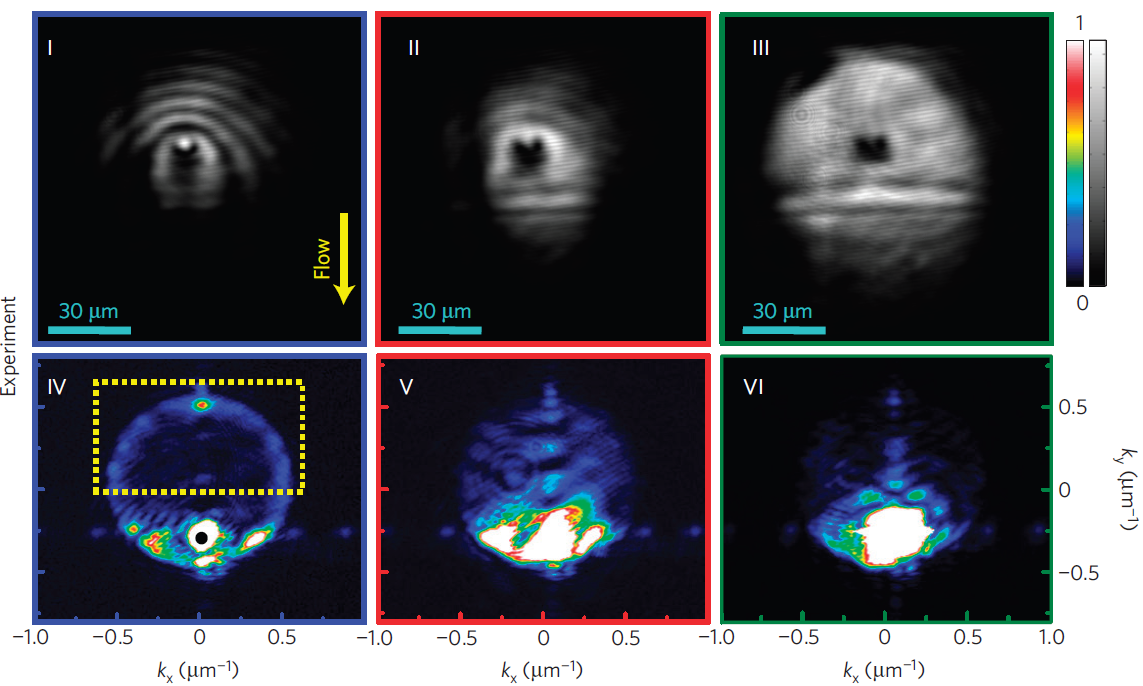
\includegraphics[width=.8\linewidth]{alberto}
  \caption{
    % 
    Experimental images of the real- (top row) and momentum- (bottom
    row) space polariton density extracted from the near/far-field light
    emitted from the cavity. The different columns correspond to
    increasing values of the polariton density, from left to right. For
    the highest density, polariton superfluidity is apparent as a
    suppression of the real-space modulation (panel III) accompanied by
    the collapse of the Rayleigh scattering ring (panel VI).
    %
    From Ref.~\cite{Amo_2009}.
    % 
  }\label{fig:alberto}
\end{figure}
% 

However, even for perturbatively weak defects, in out-of-equilibrium
systems, where the spectrum of excitations is complex, the validity of
the Landau criterion has to be
questioned~\cite{Szyma_ska_2006,Wouters_2010,Cancellieri_2010}. In the
particular case of coherently driven polaritons in the pump-only
configuration, it has been predicted~\cite{Carusotto_2004,Ciuti_2005},
and later observed~\cite{Amo_2009}, that scattering is suppressed at
either strong enough pump powers or small enough flow velocities (see
Fig.~\ref{fig:alberto}). Yet, on closer scrutiny, it has been shown
that, despite the apparent validity of the Landau criterion, the
system always experiences a residual drag force, even in the limit of
asymptotically large densities~\cite{Cancellieri_2010} or small
velocities. This result has been proven by numerically solving the
Gross-Pitaevskii equation describing the resonantly-driven polariton
system in presence of a non-perturbative extended defect. Here, the
drag force exerted by the defect on the fluid has been shown to
display a smooth crossover from the subsonic to the supersonic regime,
similar to what it has been found in the case of non-resonantly pumped
polaritons~\cite{Wouters_2010}. In this Chapter, we find an even
richer phenomenology for the dependence of the drag force on the fluid
velocity and two different kinds of crossovers from the sub- to the
supercritical regime. Furthermore, we show that the origin of the
residual drag force, which, in agreement with
Ref.~\cite{Cancellieri_2010}, lies in the polariton lifetime only, can
be demonstrated even within a linear response approximation.

More specifically, we apply the linear response theory described in
Sec.~\ref{sec:linear-response} for the case of an equilibrium
condensate and extended here to a driven-dissipative fluid in order to
analytically evaluate the drag force exerted by the coherently driven
polariton fluid in the pump-only configuration on a point-like
defect. To simplify the formalism, we restrict our analysis to the
case of resonant pumping close to the bottom of the lower polariton
dispersion, where the dispersion is quadratic. Here, the properties of
the collective excitation spectrum have been shown to be uniquely
determined by three parameters only~\cite{Ciuti_2005}: the fluid
velocity $v_p$, the interaction-renormalised pump detuning $\Delta_p$,
and the polariton lifetime $\gamma$. In particular, the sign of the
detuning $\Delta_p$ determines three qualitatively different types of
spectra: linear for $\Delta_p= 0$, diffusive-like for $\Delta_p> 0$,
and gapped for $\Delta_p< 0$.

For both cases of linear and diffusive spectra, we find a
qualitatively similar behaviour of the drag force as a function of the
fluid velocity $v_p$: In particular, the drag displays a crossover
from a subsonic or superfluid regime --- characterised by the absence
of quasiparticle excitations --- to a supersonic regime --- where
Cherenkov-like waves, similar to those of
Sec.~\ref{sec:cherenkov-emission}, are generated by the defect and
propagate into the fluid. The crossover becomes sharper for increasing
polariton lifetimes $1/\gamma$ and displays the typical threshold
behaviour for $\gamma \to 0$ with a critical velocity given by the
speed of sound of the linear regime, $v^c= c_s$, exactly as for weakly
interacting equilibrium superfluids (in the case of perturbatively
weak defects). This behaviour is similar to the one predicted for
polariton superfluids excited non-resonantly~\cite{Wouters_2010},
where the spectrum in that case is diffusive-like.

However, for gapped spectra at $\Delta_p <0$, we find that the
critical velocity governing the drag crossover exceeds the speed of
sound, $v^c > c_s$, and we determine an analytical expression of $v^c$
as a function of the detuning $\Delta_p$. Furthermore, for $\gamma \to 0$,
the drag has a threshold-like behaviour qualitatively different from
the one of weakly interacting equilibrium superfluids, with the drag
jumping discontinuously from zero to a finite value at $v_p=v^c$.

We evaluate the drag as a function of the polariton lifetime $\gamma$
and find for all three cases that: In the supercritical regime,
$v_p>v^c$, the lifetime tends to suppress the propagation of the
Cherenkov waves away from the defect and therefore to suppress the
drag. Instead, well in the subcritical regime, $v_p \ll v^c$, we find
that the residual drag goes linearly to zero with the polariton
lifetime $\gamma$, in agreement to what  was found in
Ref.~\cite{Cancellieri_2010}, by making use of a non-perturbative
numerical analysis for a finite size defect. Similar to
Ref.~\cite{Cancellieri_2010}, here, we do also find that the residual
drag in the subcritical regime can be explained in terms of an
asymmetric perturbation induced in the fluid by the defect in the
direction of the fluid velocity.

This Chapter is structured as follows: In Sec.~\ref{sec:linea} we
briefly review the linear approximation scheme and extend it to the
case of a resonantly pumped polariton fluid. We classify the three
types of collective excitation spectra in the simplified case of
excitation close to the bottom of the LP dispersion in
Sec.~\ref{sec:spect}. In Sec.~\ref{sec:drag} we derive the drag force
and characterise the crossover from the subsonic to the supersonic
regime in the three cases of zero, positive and negative detuning. In
this section, we also evaluate the drag as a function of the polariton
lifetime, interpreting therefore the results of
Ref.~\cite{Cancellieri_2010}.  Brief conclusions are drawn is
Sec.~\ref{sec:concl}.


\section{Linear response}
\label{sec:linea}

As explained in Chapter~\ref{cha:polaritons}, the description of
cavity polaritons resonantly excited by an external laser is usually
formulated in terms of a classical non-linear Schr\"odinger equation
(or Gross-Pitaevskii equation) for the LP field $\psi_{LP}(\bm{r}, t)$
(see Eq.~\eqref{eq:rspace-GPE}):
%
\begin{equation}
  i \partial_t \psi_{LP} = [\omega_{LP}(-i\nabla) - i\gamma/2 +
    V_d(\bm{r}) + g_X |\psi_{LP}|^2]\psi_{LP} + \mathcal{F}(\bm{r},t)\; .
\label{eq:basic}
\end{equation}
%
The LP dispersion is expressed in terms of the photon
$\omega_C(\bm{k}) = \omega_C(0) + \frac{\bm{k}^2}{2m_C}$ and exciton
$\omega_X(0)$ energies, the photon mass $m_C$, and the Rabi splitting
$\Omega_R$ (see Eq.~\eqref{eq:polariton-dispersion}):
%
\begin{equation}
  \omega_{LP}(\bm{k}) = \frac{1}{2} \left[\omega_C(\bm{k}) +
    \omega_X(0)\right]  - \frac{1}{2} \sqrt{\left[\omega_C(\bm{k}) -
    \omega_X(0) \right]^2 + 4\Omega_R^2} \; .
\label{eq:dispe}
\end{equation}
%
Because polaritons continuously decay at a rate $\gamma$ (see
Sec.~\ref{sec:pumping}), the cavity is replenished by a continuous
wave resonant pump $\mathcal{F}(\bm{r},t)$ at a wavevector $\bm{k}_p$ (we will
later assume $\bm{k}_p$ directed along the $x$-direction,
$\bm{k}_p = (k_p,0)$) and frequency $\omega_p$ (see
Eq.~\eqref{eq:pwpump}):
\begin{equation}
  \mathcal{F}(\bm{r},t) = f_p e^{i (\bm{k}_p \cdot \bm{r} -
    \omega_p t)} \; .
\end{equation}
%
Note that, as discussed in
Secs.~\ref{sec:lower-polaritons}--\ref{sec:mean-field},
Eq.~\eqref{eq:basic} is a simplified description of the polariton
system. It implies that the interaction nonlinearities are small
enough not to mix the lower and upper polariton branches and that we
pump far from the UP dispersion. Moreover, starting from a formulation
in terms of coupled exciton and photon fields, the polariton lifetime
would be momentum dependent and, similarly, the polariton-polariton
interaction strength $g_X$ is not contact-like as instead assumed in
Eq.~\eqref{eq:basic}. However, as shown in Appendix~\ref{app:full},
these simplifications do not affect our results qualitatively, rather,
they allow us to write them in terms of simpler
expressions. Furthermore, we have checked that, whenever the system is
excited near the bottom of the lower polariton dispersion, the results
for the drag force reported in Sec.~\ref{sec:drag} coincide with the
ones obtained using the photon-exciton coupled field description
Eq.~\eqref{eq:2-component-GPE} introduced in
Chapter~\ref{cha:polaritons}.

The potential $V_d(\bm{r})$ in Eq.~\eqref{eq:dispe} describes a
defect, which can be either naturally present in the cavity
mirror~\cite{Amo_2009} or it can be created by an additional
laser~\cite{Amo_2010}. Later on, we will assume the defect to be
point-like $V_d(\bm{r})=g_V \delta(\bm{r})$ and weak, so that we can
apply the linear response approximation~\cite{Astrakharchik_2004}.
%
As detailed in Sec.~\ref{sec:linear-response}, one divides the
response of the LP field in a mean-field component $\psi_p$
corresponding to the case when the perturbing potential is absent, and
a fluctuation part $\delta \psi (\bm{r},t)$ reflecting the linear
response of the system to the perturbing potential (see
Eq.~\eqref{eq:ansatz-atoms}):
%
\begin{equation}
  \psi_{LP} (\bm{r},t) = e^{-i \omega_p t} \left[e^{i \bm{k}_p
      \cdot \bm{r}} \psi_p + \delta \psi (\bm{r},t)\right] \; .
\label{eq:mfield}
\end{equation}
%
By substituting~\eqref{eq:mfield} into~\eqref{eq:basic}, we obtain a
mean-field equation and by retaining only the linear terms in the
fluctuation field and the defect potential, the following first order
equation in $\delta \psi (\bm{r},t)$ (the equivalent of
Eq.~\eqref{eq:GP-atoms-system}):
%
\begin{equation}
  i \partial_t \begin{pmatrix} \delta \psi \\ \delta
    \psi^* \end{pmatrix} = \hat{\mathcal{L}} \begin{pmatrix} \delta
    \psi \\ \delta \psi^* \end{pmatrix} + V_d(\bm{r}) \begin{pmatrix}
    \psi_p e^{i \bm{k}_p \cdot \bm{r}} \\ -\psi_p^{\star} e^{-i
      \bm{k}_p \cdot \bm{r}}
    \end{pmatrix}\; ,
\label{eq:linre}
\end{equation}
%
where the operator $\hat{\mathcal{L}}$ is given by (compare to
Eq.~\eqref{eq:ourL} for the atomic case):
%
\begin{equation}
 \hat{\mathcal{L}} = \begin{pmatrix} \widetilde{\omega_{LP}}
   (-i\nabla) - i \gamma/2 & g_X \psi_p^2 e^{2 i \bm{k}_p \cdot
     \bm{r}} \\ -g_X {\psi_p^{\star}}^2 e^{-2 i \bm{k}_p \cdot
     \bm{r}}& - \widetilde{\omega_{LP}}(-i \nabla) -
   i\gamma/2 \end{pmatrix}\; ,
\end{equation}
%
with $\widetilde{\omega_{LP}} = \omega_{LP}-\omega_p + 2g_X
|\psi_p|^2$. We solved the complex cubic mean-field
equation~\eqref{eq:pump-mf} for $\psi_p$ in
Sec.~\ref{sec:eq-state}. Here, we want to study the response of the
system to the presence of the defect and how different behaviours of
the onset of dissipation can be described in terms of the different
excitation spectra one can get for polaritons resonantly pumped close
to the bottom of the LP dispersion.

% mathematica nb -> dat file -> gnuplot gpi script -> eps file -> inkscape svg -> pdf file
\begin{figure}[tb]\centering
\includegraphics[width=0.75\linewidth]{dispersion} % ~/ownCloud/documents/phd_projects/point_defect_1_fluid/paper/plots/dispersion
\caption{
%
Collective excitation spectra for the subsonic (thick
solid [black] line at $v_p=0.2 c_s$, with $c_s=\sqrt{g_X|\psi_p|^2/m\sub{LP}}$)
and supersonic (dashed [red] line at $v_p=1.9 c_s$) regimes and for an
interaction-renormalised pump detuning $\Delta_p=-0.3 g_X|\psi_p|^2$ (a,
b), $\Delta_p = 0$ (c, d), $\Delta_p=0.3g_X|\psi_p|^2$ (e, f) and
$\Delta_p=2.3g_X|\psi_p|^2$ (g, h). Real parts of the spectra are
plotted in the left panels and the corresponding imaginary parts in
the right panels for $\gamma=2.2 g_X|\psi_p|^2$ --- note that in our
description the spectrum imaginary parts do not depend on the fluid
velocity $v_p$.
%
}\label{fig:spect_pmp_only}
\end{figure}
%


\subsection{Spectrum of collective excitations}
\label{sec:spect}
%
\begin{figure}[tb]\centering
  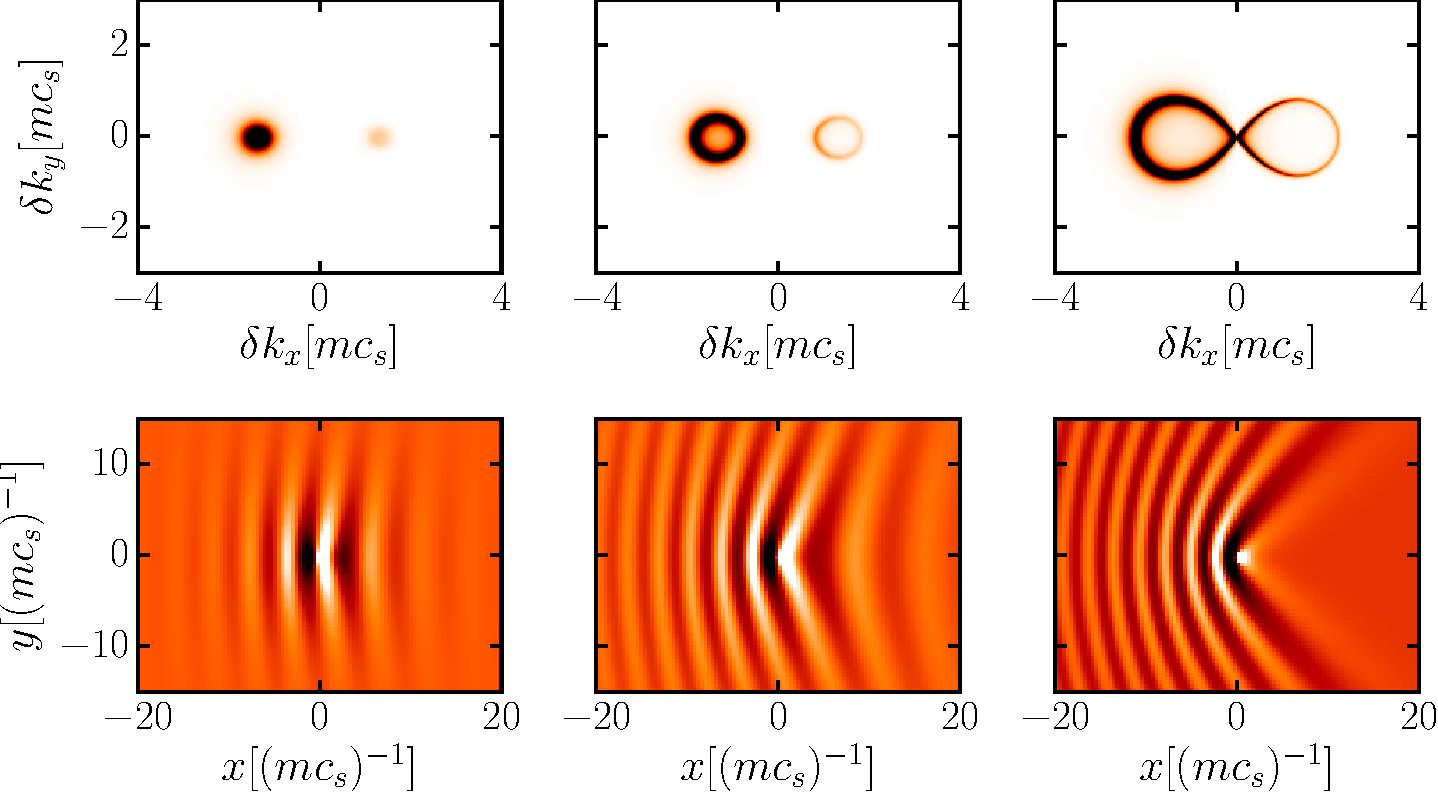
\includegraphics[width=.9\linewidth]{nond}
  % ~/ownCloud/documents/phd_projects/point_defect_1_fluid/wavefunction/julia/new_cherenkov.jl
  \caption{
    % 
    Momentum-space response (top row) $\abs{\delta \psi_s\left(\kv +
        \kv_p \right)}^2$ (arb. units) and normalised real-space
    wavefunction (bottom row) $\abs{\psi_{LP}(\rv)}^2/\abs{\psi_p}^2$
    corresponding to the nondiffusive spectra (a)--(d) in
    Fig.~\ref{fig:spect_pmp_only}. System parameters: $v_p = 1.5 c_s$,
    $\gamma = 0.06 g_X\abs{\psi_p}^2$, and $\Delta_p$ is $-0.35
    g_X\abs{\psi_p}^2$ (left column), $-0.25 g_X\abs{\psi_p}^2$ (middle
    column) and 0 (right column).
    % 
  }\label{fig:nondiffusive}
\end{figure}
%
\begin{figure}[tb]\centering
  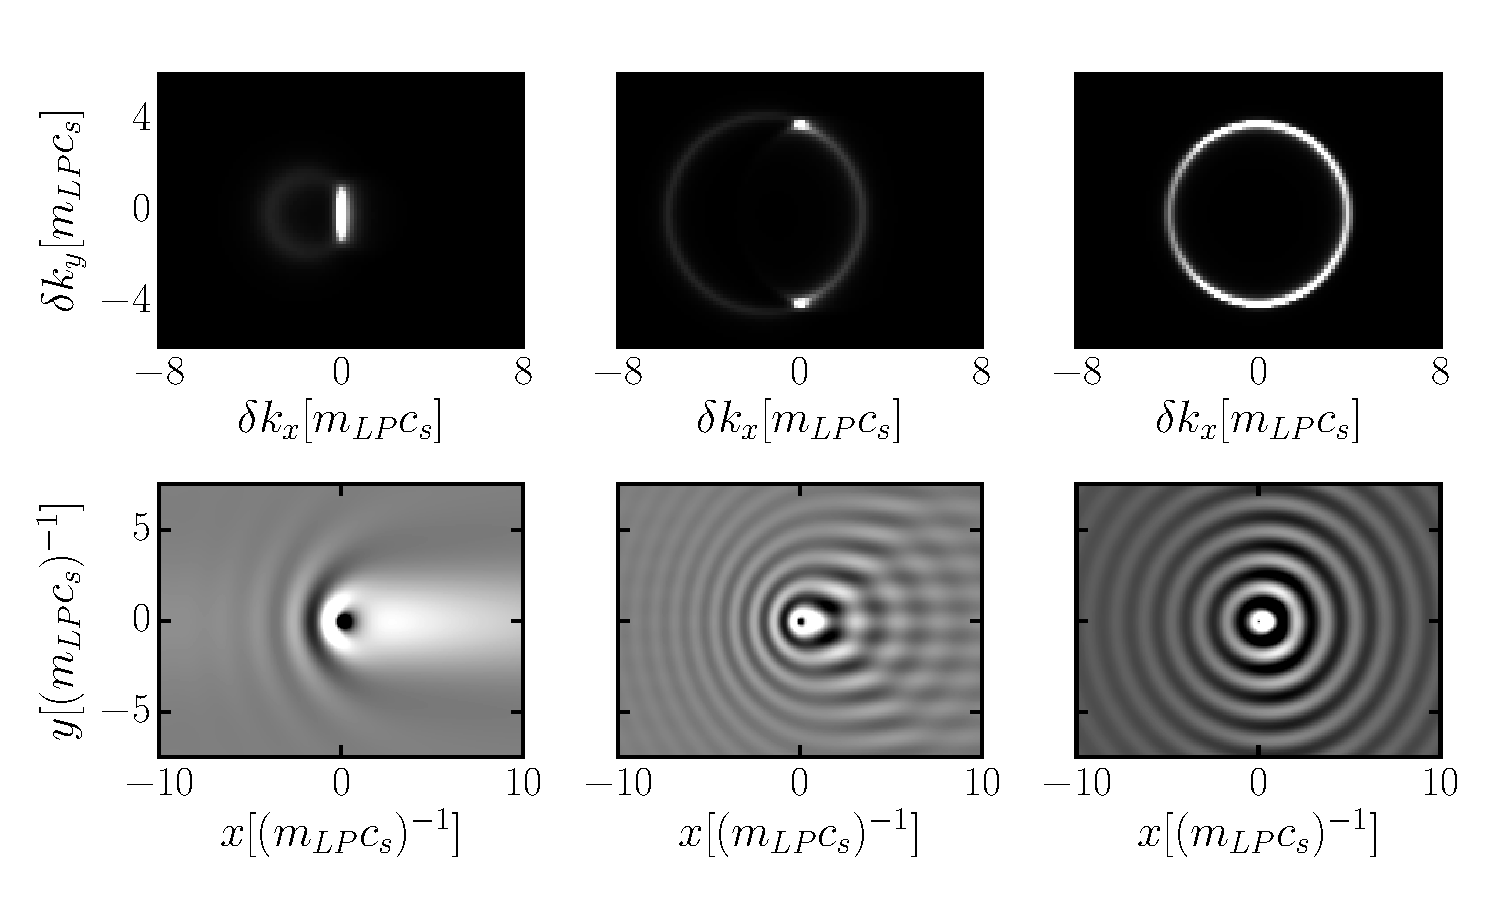
\includegraphics[width=.9\linewidth]{diff}
  % ~/ownCloud/documents/phd_projects/point_defect_1_fluid/wavefunction/julia/new_cherenkov.jl
  \caption{
    % 
    Momentum-space response (top row) $\abs{\delta \psi_s\left(\kv +
        \kv_p \right)}^2$ (arb. units) and normalised real-space
    wavefunction (bottom row) $\abs{\psi_{LP}(\rv)}^2/\abs{\psi_p}^2$
    corresponding to the diffusive spectra (e)--(h) in
    Fig.~\ref{fig:spect_pmp_only}. Polariton lifetime $\gamma = 2.2
    g_X\abs{\psi_p}^2$, and $\Delta_p = g_X\abs{\psi_p}^2$, $v_p = 1.5 c_s$
    (left column); $\Delta_p = 9 g_X\abs{\psi_p}^2$, $v_p = 1.5 c_s$ (middle
    column) and $\Delta_p = 9 g_X\abs{\psi_p}^2$, $v_p = 0.07 c_s$ (right
    column).
    % 
  }\label{fig:diffusive}
\end{figure}
%
The spectrum of the collective excitations can be obtained by
diagonalising the operator $\hat{\mathcal{L}}$ in the momentum space
representation, following the approach of
Sec.~\ref{sec:cherenkov-emission} (see Eq.~\eqref{eq:translated-L})
%
\begin{equation}
  \mathcal{L}_{\bm{k},\bm{k}_p} = \begin{pmatrix}
    \widetilde{\omega_{LP}} (\delta \bm{k}+\bm{k}_p) - i \gamma/2 &
    g_X \psi_p^2 \\ -g_X {\psi_p^{\star}}^2 & -
    \widetilde{\omega_{LP}}(\delta \bm{k}-\bm{k}_p) -
    i\gamma/2 \end{pmatrix}\; ,
\label{eq:opell}
\end{equation}
%
where, $\delta \bm{k} = \bm{k} - \bm{k}_p$. The description of the
spectrum simplifies in the case when the pumping is close to the
bottom of the LP dispersion, that can be approximated as parabolic
(see Eq.~\eqref{eq:parabolic-disp})
%
\begin{equation}
  \omega_{LP} (\delta \bm{k} \pm \bm{k}_p) \simeq \omega_{LP}(0) +
  \frac{k_p^2}{2m\sub{LP}} + \frac{\delta \bm{k}^2}{2m\sub{LP}} \pm \delta \bm{k}
  \cdot \bm{v}_p \; ,
\end{equation}
%
where $\bm{v}_p=\bm{k}_p/m\sub{LP}$ is the fluid velocity, and
$m\sub{LP}$ is the LP mass of Eq.~\eqref{eq:LP-mass}. This
simplification allows one to describe the complex spectrum in terms of
three parameters only, namely the fluid velocity $\bm{v}_p$, the
interaction-renormalised pump detuning (defined in
Sec.~\ref{sec:eq-state})
%
\begin{equation}
  \Delta_p = \omega_p - \left[\omega_{LP} (0) +\frac{k_p^2}{2m\sub{LP}} +
    g_X|\psi_p|^2\right]
\end{equation}
%
and the LP lifetime $\gamma$. One observation we can immediately make
is that, unlike the atomic case, one will no longer have a sharp
corner\footnote{Unless, of course, $\Delta_p = 0$.}  in the spectrum
at $\delta \bm{k} = 0$, as that feature depended on the equality (up
to a sign) between the diagonal and off-diagonal elements of
$\mathcal{L}$.
%
The elementary excitation spectrum of coherently-driven polaritons
reads (compare this to the spectrum given by
Eq.~\eqref{eq:boosted-bogoliubov}):
%
\begin{equation}
  \omega_{\pm} (\bm{k}) = \delta \bm{k}\cdot \bm{v}_p - i\gamma/2
  \pm \sqrt{\varepsilon(\delta \bm{k}) \left[\varepsilon(\delta
      \bm{k}) + 2g_X|\psi_p|^2\right]} \; ,
\label{eq:spect}
\end{equation}
%
where $\varepsilon(\bm{k}) = \frac{k^2}{2m\sub{LP}} - \Delta_p$. If energies
are measured in units of the mean-field energy blue-shift $g_X
|\psi_p|^2$ (we will use the notation $\Delta_p' =
\Delta_p/g_X|\psi_p|^2$ and $\gamma'= \gamma/g_X|\psi_p|^2$), then the
fluid velocity $v_p$ is measured in units of the speed of sound $c_s =
\sqrt{g_X|\psi_p|^2/m\sub{LP}}$. In order to make connection with the current
experiments, note that, for blue-shifts in the range $g_X |\psi_p|^2
\simeq 0.1-1$~meV, typical values of the speed of sound $c_s$ are
$0.8-2.7\times 10^6$~m/s. Similarly, for common values of the LP mass,
the range in momenta in Fig.~\ref{fig:spect_pmp_only} comes of the order of
$\delta k_x \simeq 0.2-0.8$~$\mu$m${}^{-1}$.

%
\begin{figure}[tb]\centering
  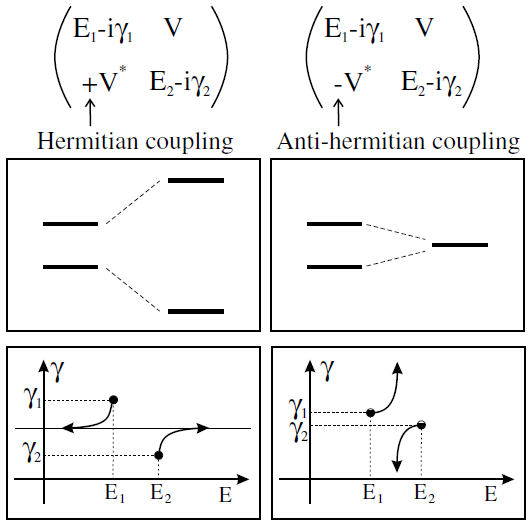
\includegraphics[width=.6\linewidth]{branch_sticking}
  \caption{
    % 
    Hermitian (left column) and anti-Hermitian (right column) coupling
    between two damped oscillators of energies $E_1$, $E_2$, decay rates
    $\gamma_1$, $\gamma_2$ and interaction energy $V$. Top row shows the
    coupling matrices, while middle (bottom) row shows the evolution of
    the real (complex) eigenvalues, with increasing $\abs{V}$. From
    Ref.~\cite{Ciuti_2003}.
    % 
  }\label{fig:branch-stick}
\end{figure}
% 

The spectrum~\eqref{eq:spect} can be classified according to the sign
of the interaction-renormalised pump detuning
$\Delta_p$~\cite{Carusotto_2004,Ciuti_2005} --- see
Fig.~\ref{fig:spect_pmp_only}. For $\Delta_p<0$ (panels [a,b]), the
real part of the spectrum lacks the sonic behaviour at small
$\delta \kv$, and shows a \emph{gap} that increases with
$\abs{\Delta_p}$, while the imaginary part is determined by the
polariton lifetime $\gamma$ only.
%
If one applies the Landau criterion for the real part
of the spectrum only, then one finds a critical velocity
%
\begin{equation}
  \frac{v^c}{c_s} = \sqrt{1 + |\Delta_p'| +
    \sqrt{|\Delta_p'|(|\Delta_p'| + 2)}} > 1\; ,
\label{eq:criti}
\end{equation}
%
always larger than the speed of sound for $\Delta_p<0$. 
%
If the fluid velocity is subcritical, $v_p<v^c$ (see the [black] solid
lines in Fig.~\ref{fig:spect_pmp_only}(a)), then no quasiparticles can
be excited and thus, for infinitely living polaritons $\gamma \to 0$,
the fluid would experience no drag when scattering against the
defect. 
%
For the case of $v_p = v^c$, the $\Re[\omega_{+}(\bm{k})]$ branch
touches the $\omega = 0$ plane in one point (see left column of
Fig.~\ref{fig:nondiffusive}), resulting in a localized perturbation
around the defect, with an additional stripe pattern of wavevector
$m\sub{LP}v^c$, caused by the interference of the pump with the momentum of
the scattered state.
%
For supercritical velocities instead, $v_p > v^c$ see the [red] dashed
lines in Fig.~\ref{fig:spect_pmp_only}(a), one expects dissipation in
the form of radiation of Cherenkov-like waves from the defect into the
fluid. In the supercritical regime, the set of wavevectors $\bm{k}$
for which $\Re[\omega_{+} (\bm{k})] = 0$ form a closed curve in
$\bm{k}$-space with no singularity of the derivative (see middle
column of Fig.~\ref{fig:nondiffusive}). As explained in the
geometrical model presented in Sec.~\ref{sec:cherenkov-emission}, this
means the radiation can be emitted in all possible directions around
the defect. This, as we will see in the next section, will imply that
the drag force for $\gamma \to 0$ goes abruptly, rather than
continuously, from zero at $v_p<v^c$ to a finite value at
$v_p \ge v^c$.

The spectrum gap closes to zero in the resonant situation at
$\Delta_p=0$, when the two branches $\omega_{\pm} (\bm{k})$ touch at
$\delta \bm{k}=0$ (panels [c,d] of Fig.~\ref{fig:spect_pmp_only}).
%
Here, the real part of the spectrum displays the standard \emph{sonic
  dispersion} at small wavevectors (as for the weakly interacting
bosonic gases of Chapter~\ref{cha:cold-gases}) with a slope given by
$c_s \pm v_p$. The imaginary part, as in the previous case, is
constant and equal to $-\gamma/2$. It is clear therefore that in this
case, when $\gamma \to 0$, one recovers the equilibrium results valid
for weakly interacting gases~\cite{Astrakharchik_2004,Carusotto_2006},
where the critical velocity for superfluidity equals the speed of
sound, $v^c=c_s$, and the drag displays a threshold-like
behaviour. Here, in the supersonic regime $v_p > v^c$, the closed
curve $\Re[ \omega_{+} (\bm{k})] = 0$ has instead a singularity,
resulting in the standard Mach cone of aperture $\theta$, $\sin \theta
= c_s/v_p$, inside which radiation from the defect cannot be
emitted~\cite{Carusotto_2006} (see right column of
Fig.~\ref{fig:nondiffusive}, as well as Fig.~\ref{fig:bogo-cherenkov}
of Sec.~\ref{sec:cherenkov-emission}).

For $\Delta_p > 0$, the real parts of the two Bogoliubov branches
cross and stick together, giving rise to flat regions near the
crossing points. This is due to level attraction caused by the
anti-Hermitian coupling of Eq.~\eqref{eq:opell}, and is accompanied
by a splitting of the imaginary parts, as illustrated in
Fig.~\ref{fig:branch-stick}. We further distinguish two separate
cases, $0 < \Delta_p \le 2$ and $\Delta_p > 2$.
%
In the first case (panels [e,f]), there is only one flat region in
momentum-space, and the intensity of the Rayleigh scattering is
amplified on a segment situated at $\delta k_x = 0$ and oriented
parallel to the $y$ axis, as shown in the left column of
Fig.~\ref{fig:diffusive}. A consequence of this (parametric)
amplification is the long shadow seen in the real-space
image~\cite{Ciuti_2005}. As the imaginary part only has one peak
(corresponding to the pump), this is the precursor of the Kerr
single-mode instability described in Sec.~\ref{sec:eq-state}.
%
The second case (panels [g,h]) has a different momentum-space
topology, with two flat regions, producing two distinct peaks in the
imaginary part. As soon as these become positive, one enters the
regime of parametric oscillation (see Sec.~\ref{sec:opo}), with the
signal and idler momenta situated at the two maxima. The corresponding
far-field image plotted in the middle column of
Fig.~\ref{fig:diffusive} shows two pronounced peaks on the line
passing through $\delta k_x = 0$, the interference of which results in
a near-field ``zebra-like'' pattern~\cite{Ciuti_2005}. For very small
fluid velocities (see right column of Fig.~\ref{fig:diffusive}), the
two Bogoliubov branches cross on a ring of wavevectors, giving rise to
cylindrical wavefronts~\cite{Van_Regemortel_2014}.
%
We note that spectra [e]--[h] have no correspondence in equilibrium
systems, because a finite polariton lifetime $\gamma$ is needed in
order to insure stability, $\Im[\omega_{\pm}(\bm{k})]<0$. Following
the literature~\cite{Carusotto_2013}, we refer to these spectra as
\emph{diffusive-like}.
%
We also note that, for these spectra, even if considering only the
real part of the collective excitation spectrum, as soon as the fluid
is in motion, dissipation in the form of waves is possible.
%
However, we will see that, similar to the case of non-resonantly
pumped polaritons~\cite{Wouters_2010}, when decreasing $\gamma$ (and
accordingly $\Delta_p$ in order to have stable solutions), this
situation continuously connects to the case where a threshold-like
behaviour with $v^c = c_s$ was found.

%%
We will see in the next section how these different spectra imply only
two qualitatively different types of crossover of the drag force as a
function of the fluid velocity, for either $\Delta_p < 0$ or
$\Delta_p \ge 0$ pump detunings.

%
\begin{figure}[tb]\centering
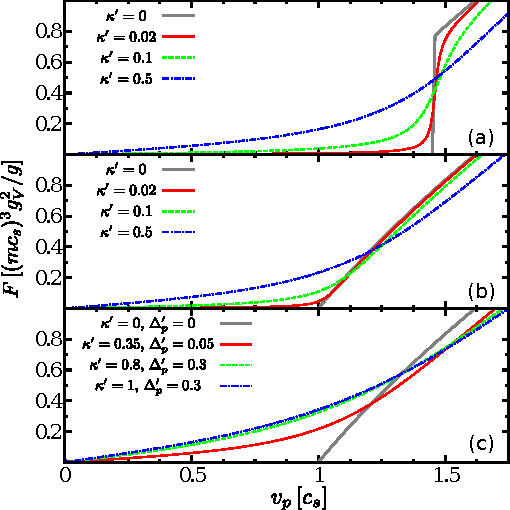
\includegraphics[width=0.6\linewidth]{dragspeed} % ~/ownCloud/documents/phd_projects/point_defect_1_fluid/paper/plots/dragspeed
\caption{
%
Drag force $F_d$ as a function of the fluid velocity
$v_p$ for different values of the pump detuning $\Delta_p$:
$\Delta_p=-0.3g_X|\psi_p|^2$ (a), $\Delta_p=0$ (b), and $\Delta_p>0$
(c), and for different values of the polariton lifetime --- here, we
use the notation $\gamma' = \gamma/g_X|\psi_p|^2$ and $\Delta_p' =
\Delta/g_X|\psi_p|^2$.
%
}\label{fig:dragv}
\end{figure}


\section{Drag force}
\label{sec:drag}
%
The steady state response of the system to a static and weak defect
can be evaluated starting from Eq.~\eqref{eq:linre}:
%
\begin{equation*}
  \begin{pmatrix} \delta \psi_s(\bm{r}) \\ \delta
    \psi_s^*(\bm{r}) \end{pmatrix} =
  \hat{\mathcal{L}}^{-1} \begin{pmatrix} V_d(\bm{r}) e^{i \bm{k}_p
      \cdot \bm{r}} \psi_p \\ -V_d(\bm{r}) e^{-i \bm{k}_p \cdot
      \bm{r}} \psi_p^{\star} \end{pmatrix} \; .
\end{equation*}
%
For a point-like defect, this can be written in momentum space as:
%
\begin{equation*}
  \delta \psi_s (\bm{k} + \bm{k}_p) = \frac{-g_V \psi_p
    (\varepsilon(\bm{k}) - \bm{k} \cdot \bm{v}_p +
    i\gamma/2)}{\varepsilon(\bm{k}) [\varepsilon(\bm{k}) +
      2g_X|\psi_p|^2] - (\bm{k} \cdot \bm{v}_p - i\gamma/2)^2} \; ,
\end{equation*}
%
while the other component $\delta \psi_s^* (\bm{k}_p - \bm{k})$ can be
obtained by complex conjugation and by substituting
$\bm{k} \rightarrow -\bm{k}$. The drag force exerted by the defect on the
fluid is given by the expectation value of the operator
$-\bm{\nabla}V_d(\bm{r})$ over the condensate
wavefunction~\cite{Pavloff2002}:
%
\begin{equation}
  \bm{F}_d = - \int d\bm{r} |\psi_{LP}(\bm{r},t)|^2 \bm{\nabla}V_d(\bm{r}) \; ,
\end{equation}
%
This definition is justified for conservative systems in
Appendix~\ref{app:field-theory}, using the momentum-flux tensor. In
the steady state linear response regime, we obtain:
%
\begin{multline}
  \bm{F}_d = g_V \int \frac{d\bm{k}}{(2\pi)^2} i\bm{k}
  \left[\psi_p^* \delta\psi_s (\bm{k} + \bm{k}_p) + \psi_p \delta
    \psi_s^* (\bm{k}_p - \bm{k})\right]\\
%
  = 2g_V^2|\psi_p|^2 \int \frac{d\bm{k}}{(2\pi)^2} \frac{i\bm{k}
    \varepsilon(\bm{k})}{\omega_{+} (\bm{k})\omega_{-} (\bm{k})}
  \; .
    \label{eq:dragf}
\end{multline}
%
The drag is clearly oriented along the fluid velocity $\bm{v}_p$,
i.e., $\bm{F}_d = F_d \hat{\bm{v}}_p$. If $\gamma \to 0$, then the
integral in Eq.~\eqref{eq:dragf} is finite only if poles exist when
$\Re [\omega_{\pm} (\bm{k})] = 0$, i.e., when quasiparticles can be
excited, in agreement with the Landau criterion. For finite polariton
lifetimes, however, it is clear that the integral will always be
different from zero for $v_p>0$.
% Note that the only dependence on the polariton lifetime $\gamma$ is
%in the denominator of the integral in Eq.~\eqref{eq:dragf}.
We now analyse the behaviour of the drag force as a function of the
fluid velocity for the three ($\Delta_p = 0$, $\Delta_p > 0$, and
$\Delta_p < 0$) different spectra illustrated in the previous section.

\begin{figure}[tb]\centering
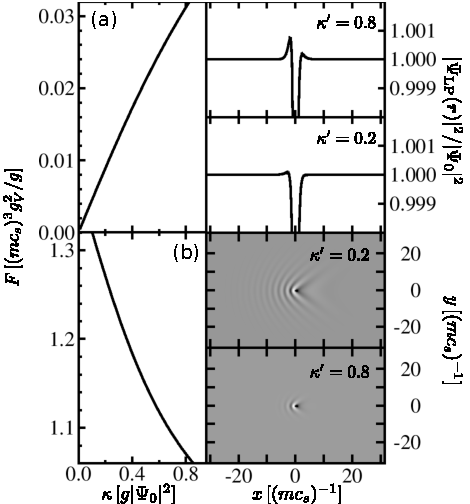
\includegraphics[width=0.6\linewidth]{dragkappa}
% ~/ownCloud/documents/phd_projects/point_defect_1_fluid/paper/plots/kappa
%% ~/ownCloud/documents/phd_projects/point_defect_1_fluid/wavefunction/python/cerenkov.py
\caption{
%
Drag force $F_d$ as a function of the inverse polariton
lifetime $\gamma'=\gamma/(g_X |\psi_p|^2)$ in the (a) subcritical regime
($v_p=0.2 c_s$) and (b) supercritical regime ($v_p=1.9 c_s$). In both
cases we have fixed $\Delta_p=-0.3g_X|\psi_p|^2$ ($v^c \simeq 1.46 c_s$)
but these results are qualitatively similar for any other value of the
pump detuning. We plot in the right panels the normalised real-space
wavefunction $|\psi_{LP}(\bm{r})|^2/|\psi_p|^2$ for two specific
values of $\gamma'=0.4$ and $\gamma'=1.6$.
%
}\label{fig:dragk}
\end{figure}

For the \emph{linear} spectrum, at $\Delta_p=0$, in the equilibrium
limit, $\gamma \to 0$, we recover for the drag the known result of
weakly interacting Bose gases in two
dimensions~\cite{Astrakharchik_2004}:
%
\begin{equation}
  \frac{F_d}{(m\sub{LP}c_s)^3 g_V^2/g_X}=\frac{(v_p/c_s)^2 - 1}{v_p/c_s}
  \Theta(v_p - c_s)\; ,
\label{eq:drag0}
\end{equation}
%
with a threshold-like behaviour at a critical fluid velocity equal to
the speed of sound $c_s$. This limiting result is plotted as a bold
gray line in the panels (b,c) of Fig.~\ref{fig:dragv}. For
$\Delta_p=0$ and finite lifetimes $\gamma$, we find a smooth crossover
from the subsonic to the supersonic regime, with the drag being closer
to the equilibrium threshold behaviour for decreasing $\gamma$ (see
Fig.~\ref{fig:dragv}(b)). A finite lifetime tends to increase the
value of the drag in the subsonic region $v_p \ll v^c$, giving place
to a residual drag force, similar to what was found in the numerical
simulations of Ref.~\cite{Cancellieri_2010} (see
Fig.~\ref{fig:emiliano}). Instead, in the supersonic region
$v_p \gg v^c$, the finite lifetime tends to decrease the value of the
drag. 

In the case of \emph{diffusive-like} spectra at $\Delta_p>0$ the
situation is qualitatively very similar to the resonant case (see
Fig.~\ref{fig:dragv}(c)), with the difference that now, in order to
have stable solutions, we can decrease the value of the lifetime only
by decreasing accordingly also the value of the pump detuning
$\Delta_p$. The crossover for both $\Delta_p = 0$ and $\Delta_p > 0$
is also qualitatively very similar to the case of non-resonantly
pumped polaritons~\cite{Wouters_2010}, where the spectrum of
excitation is diffusive-like. In Ref.~\cite{Larr__2012}, a similar
approach was used to analytically derive the drag for nonresonantly
pumped polaritons in 1D, finding a continuous crossover from a regime
dominated by viscous drag (of Stokes type) to one dominated by wave
resistance. Futhermore, the authors proved that it was not possible to
separate the viscous and wave-resistance components of the drag.
Shortly after the publication of Ref.~\cite{Berceanu_2012} (on which
this Chapter is based), Van Regemortel et
al.~\cite{Van_Regemortel_2014} found that the parametric amplification
mechanism described in Sec.~\ref{sec:spect} can increase the
scattering of particles in the flow direction (for low condensate
speeds), leading to a \emph{negative drag force}, i.e. a force
directed opposite to the flow direction. To see how this comes about,
one can look at the right column of Fig.~\ref{fig:diffusive}: the top
panel shows that the average momentum of the scattered modes is in the
positive $\delta k_x$ direction. This, in turn, leads to a pileup of
the fluid density behind the defect ($x > 0$), as can be seen in the
bottom panel.

\begin{figure}[tb]\centering
  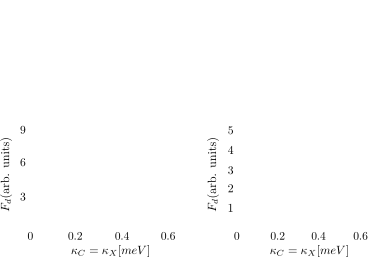
\includegraphics[width=.7\linewidth]{emiliano}
  \caption{
    % 
    \emph{Top row}: Photon density along $y=0$, perturbed by a
    circular potential of radius $7$ $\mu$m and height 110 meV (centered
    at the origin), in the subcritical regime. The pump momentum is $k_p =
    1$ $\mu$m${}^{-1}$, and the panels (from left to right) correspond to
    decreasing exciton ($\gamma_X$) and photon ($\gamma_C$) decay rates
    $\gamma_X = \gamma_C =$ 1.3, 0.44 and 0.011 meV. 
    % 0.6582119/(x [ps]) = \gamma/2 [meV]
    %
    \emph{Bottom row}: Residual drag force as a function of decay
    rate. The left panel compares two different values of $k_p$, namely
    0.7 (black solid line) and 1 $\mu$m${}^{-1}$ (red dashed line). The
    right panel shows two different potential heights, of -22 (blue
    dashed line) and -2.2 meV (red dashed line), with $k_p = 0.7$
    $\mu$m${}^{-1}$.
    %
    In all plots, the pump is 0.44 meV blue-detuned above the bare LP
    branch $\omega_{LP}(\kv_{p})$. Adapted from
    Ref.~\cite{Cancellieri_2010}.
    % 
  }\label{fig:emiliano}
\end{figure}

In the case of \emph{gapped} spectra, the situation is, however,
qualitatively different (see Fig.~\ref{fig:dragv}(a)). For infinitely
living polaritons, $\gamma \to 0$, the drag force can also be
evaluated analytically and its expression is similar to
Eq.~\eqref{eq:drag0}, but with a critical velocity larger than the
speed of sound, the expression of which is given in
Eq.~\eqref{eq:criti}:
%
\begin{equation}
  \frac{F_d}{(m\sub{LP}c_s)^3 g_V^2/g_X}=\frac{(v_p/c_s)^2 - 1}{v_p/c_s}
  \Theta(v_p - v^c)\; .
\end{equation}
%
Therefore now the drag experiences a jump for $v_p=v^c$, rather than a
continuous threshold as for the resonant case $\Delta_p=0$. As already
mentioned in the previous section, this discontinuous behaviour of the
drag for the gapped spectra is connected to the fact that, as soon as
quasiparticles can be excited by the defect at $v_p\ge v^c$,
Cherenkov-like waves can be immediately emitted in all directions,
rather than being restricted in a region outside the Mach cone as
before. For $\Delta_p=0$, the cone was gradually closing with
increasing  fluid velocity.

Both the increase of the value of the drag in the subcritical region
as a function of the polariton lifetime and the decrease in the
supercritical region, are behaviours common to all the types of
spectra. We plot the drag force as a function of $\gamma$ in
Fig.~\ref{fig:dragk}, for two values of the fluid velocity $v_p$ and a
specific value of the pump detuning $\Delta_p$, though we have checked
that the following results are generic. For $v_p < v^c$, we find that
the residual drag is a finite-lifetime effect only and, well below the
critical velocity, the drag force goes linearly to zero for
$\gamma \to 0$. This is in agreement with the results of
Ref.~\cite{Cancellieri_2010}, where the full GP equation for the
coupled exciton and photon fields was solved numerically for a
finite-size defect: see the bottom row of Fig.~\ref{fig:emiliano} for
the numerical drag in the limit of asymptotically large densities.

In the resonant case $\Delta_p=0$, the slope of the
drag for $v_p \ll c_s$ can be evaluated analytically starting from the
expression~\eqref{eq:dragf}:
%
\begin{equation*}
    \frac{F_d}{(m\sub{LP}c_s)^3 g_V^2/g_X} \mathop{\simeq}\limits_{\gamma \to 0} \frac{2 c_s}{\pi
      v_p} \left( \frac{1}{ \sqrt{1-(v_p/c_s)^2}} - 1 \right)
    \frac{\gamma}{2g_X |\psi_p|^2} \; .
\end{equation*}
%
The residual drag in the subsonic regime is an effect of the
broadening of the quasi-particles energies: Even when the spectrum
real part does not allow any scattering against the defect (e.g., for
$\Delta_p \le 0$), the broadening produces some scattering close to
the defect. This results in a perturbation of the fluid around the
defect, asymmetric in the direction of the fluid velocity (see panel
(a) of Fig.~\ref{fig:dragk}), similar to what was obtained in
Ref.~\cite{Cancellieri_2010} (see top row of
Fig.~\ref{fig:emiliano}). Instead, in the supersonic regime, the drag
force is weaker in the non-equilibrium case with respect to the
equilibrium one. This is caused by the finite lifetime tending to
suppress the propagation of the Cherenkov waves away from the defect,
as shown in panel (b) of Fig.~\ref{fig:dragk}.


\section{Conclusions and discussion}
\label{sec:concl}
%
To conclude, we have analysed the linear response to a weak defect of
resonantly pumped polaritons in the pump-only state, and we have been
able to determine two different kinds of threshold-like behaviours for
the drag force as a function of the fluid velocity. In the case of
either zero or positive pump detuning, one can continuously connect to
the case of equilibrium weakly interacting gases of
Chapter~\ref{cha:cold-gases}, where the drag displays a continuous
threshold with a critical velocity equal to the speed of
sound. However, for negative pump detuning, where the spectrum of
excitations is gapped, the drag shows a discontinuity with a critical
velocity larger than the speed of sound. In this sense, the case of
coherently driven microcavity polaritons in the pump-only
configuration displays a richer phenomenology than the case of
nonresonantly pumped polariton superfluids. We have also seen that the
absence of a long-range wake does not imply the absence of
dissipation, as a residual drag force due to the finite polariton
lifetime is always present in the system. In this sense, one can say
that we are not dealing with superfluid behaviour in a strict sense.

\begin{subappendices}
\section{GP equation for the LP branch}
\label{app:full}
%
If one starts from a description of polaritons in terms of separate
exciton and cavity photon fields, a rotation into the LP and UP basis,
followed by neglecting the occupancy of the upper polariton branch, as
explained in detail in Chapter~\ref{cha:polaritons}, results in the
following Gross-Pitaevskii equation (compare to
Eq.~\eqref{eq:mom-GPE}) for the LP field in momentum space
$\psi_{LP}(\bm{r},t) = \sum_{\bm{k}} e^{i\bm{k}\cdot \bm{r}}
\psi_{LP,\bm{k}} (t)$~\cite{Ciuti_2003}:
%
\begin{multline}
  i\partial_t \psi_{LP,\bm{k}} = f_p e^{-i\omega_p t}
  \delta_{\bm{k},\bm{k}_p} + \left[\omega_{LP} (\kv) - i\gamma
    (\kv)/2\right]\psi_{LP,\bm{k}} +\\
%
  \sum_{\bm{k}_1, \bm{k}_2} g_{\bm{k}, \bm{k}_1, \bm{k}_2}
  \psi^*_{LP,\bm{k}_1 + \bm{k}_2-\bm{k}} \psi_{LP,\bm{k}_1}
  \psi_{LP,\bm{k}_2} + C_{\kv} \sum_{\bm{k}_1} V_{d,{\bm{k} - \bm{k}_1}} \psi_{LP,\bm{k}_1} C_{\kv_1}\; ,
\end{multline}
%
where $\gamma(\kv)=\gamma_X X^2_{\kv} + \gamma_C C^2_{\kv}$ is the effective LP
decay rate,
%
\begin{equation}
  g_{\bm{k}, \bm{k}_1, \bm{k}_2}=g_X X_{\kv}X_{|\bm{k}_1 + \bm{k}_2-\bm{k}|} X_{\kv_1} X_{\kv_2}
\end{equation}
%
is the interaction strength, and where
$V_d(\bm{r}) = \sum_{\bm{k}} e^{i\bm{k}\cdot \bm{r}} V_{d,{\bm{k}}}$.

In these expressions, the coefficients (see Eqs.~\eqref{eq:hopfield-X}
and~\eqref{eq:hopfield-C}) 
%
\begin{equation}
  X^2_{\kv}, C^2_{\kv} = \frac{1}{2} \left(1 \pm \frac{\omega_C(\kv) -
    \omega_X(0)}{\sqrt{(\omega_C(\kv) - \omega_X(0))^2 +
      4\Omega_R^2}}\right)
\end{equation}
%
are the Hopfield coefficients used to diagonalise the free polariton
Hamiltonian. We want here to justify the simplified description done
in Eq.~\eqref{eq:basic}. If we follow the linear response expansion as
in~\eqref{eq:mfield}, the operator $\hat{\mathcal{L}}$ in momentum
space analogous to~\eqref{eq:opell} reads as:
%
\begin{equation}
  \mathcal{L}_{\bm{k},\bm{k}_p} = \begin{pmatrix}
    \widetilde{\omega_{LP}} (\delta \bm{k}+\bm{k}_p) - i
    \gamma(\delta \bm{k}+\bm{k}_p)/2 & g_X X_{\kv_p}^2 X_{\delta
      \bm{k}+\bm{k}_p} X_{\delta \bm{k}-\bm{k}_p} \psi_p^2
    \\ - g_X X_{\kv_p}^2 X_{\delta \bm{k}+\bm{k}_p} X_{\delta
      \bm{k}-\bm{k}_p}{\psi_p^{\star}}^2 & -
    \widetilde{\omega_{LP}}(\delta \bm{k}-\bm{k}_p) -
    i\gamma(\delta \bm{k}-\bm{k}_p)/2 \end{pmatrix}\; ,
\label{eq:opel2}
\end{equation}
%
where now $\widetilde{\omega_{LP}} (\delta \bm{k} \pm\bm{k}_p) =
\omega_{LP} (\delta \bm{k} \pm\bm{k}_p) -\omega_p + 2 g_X X_{\kv_p}^2
X_{\delta \bm{k} \pm \bm{k}_p}^2 |\psi_p|^2$. It is easy to show that
the eigenvalues of this operator coincide with our approximated
expressions~\eqref{eq:spect} in the limit of $\delta k \ll k_p$,
when $X_{\delta \bm{k} \pm \bm{k}_p}^2 \simeq X_{\kv_p}^2$, $C_{\delta
\bm{k} \pm \bm{k}_p}^2 \simeq C_{\kv_p}^2$ and when we can simply
rename $g_X \equiv g_X X_{\kv_p}^4$ and $\gamma \equiv
\gamma(\kv_p)$. It is interesting to note that, even if we would
retain the linear terms in $\bm{k}_p \cdot \delta \bm{k}$ in the
expansion of $X_{\delta \bm{k} \pm \bm{k}_p}^2$, this would result in
a renormalisation of the fluid velocity $\bm{v}_p$ in the
expression~\eqref{eq:spect} which takes into account the blue-shift of
the LP dispersion due to the interaction.
\end{subappendices}


%%% Local Variables:
%%% mode: latex
%%% TeX-master: "../thesis_berceanu"
%%% End:
